\chapter{Parte IV - Apresentações e Pôsteres}
\label{cap:parteIV}

\section{Pacote Beamer}
\label{sec:beamer}

O \textit{Beamer} é o pacote padrão do \LaTeX{} para a produção de apresentações no estilo do \textit{Microsoft PowerPoint}. Assim como os documentos do \LaTeX{}, é possível reconhecer os documentos de apresentações produzidos pelo \textit{Beamer} pela sua qualidade gráfica e pelos seus estilos pré-definidos (embora seja possível criar estilos a partir do zero, esta tarefa não será abordada aqui).

Um documento do \textit{Beamer} é tão simples quanto um documento do \LaTeX{}. Ele é uma classe de documentos, então para criar um documento \textit{Beamer}, basta utilizar esta classe. Veja no Exemplo \ref{exe:beamer1} a seguir, um exemplo mínimo.

\begin{texexptitled}[breakable,center lower,enhanced jigsaw,middle=2mm,listing side comment,righthand width=5.5cm,compilable listing,run latex,run dvips,run ps2pdf,pdf comment,comment style={raster columns=1},freeze pdf]{Um documento \textit{Beamer} mínimo}{exe:beamer1}
\documentclass{beamer}
\usepackage[utf8]{inputenc}
\usepackage{lipsum}

\title{Título}
\author{Nome}
\date{September 2019}

\begin{document}

\maketitle

\section{Seção}

\subsection{Subseção}

\begin{frame}{Frame}
\lipsum[1]
\end{frame}

\end{document}
\end{texexptitled}

Diferente de um documento \LaTeX{} mínimo, como aquele mostrado no Exemplo \ref{exe_doc}, um documento do \textit{Beamer} contém \textit{frames}, que são inseridas com o ambiente padrão {\tt frame}. Um \textit{frame} é um como um \textit{slide} do \textit{Microsoft PowerPoint} e dentro dele é possível inserir qualquer tipo de outros ambientes que normalmente são inseridos dentro de um documento \LaTeX{} comum, e.g., listas, figuras, tabelas, textos e duas ou mais colunas, \textit{minipages}, \textit{listings} e outros.

Nas seções a seguir, são mostradas alguns detalhes de alguns dos elementos principais de um documento \textit{Beamer}.

\subsection{Estilos}
\label{sec:estilos}

Assim como qualquer outro editor de apresentações, no \textit{Beamer} também é possível utilizar estilos e aplicar diferentes estilos nas fontes do documento. O estilo de um documento \textit{Beamer} é definido através tema, esquema de cores e estilo de fontes. Para isto, utilizam-se os comandos a seguir no preâmbulo de um documento \textit{Beamer}:

\begin{itemize}
    \item \mintinline{latex}{\usetheme}
    \item \mintinline{latex}{\setbeamercolor}
    \item \mintinline{latex}{\usefonttheme}
\end{itemize}

O comando \mintinline{latex}{\usetheme} define um dos 26 temas predefinidos do \textit{Beamer}. O esquema de cores padrão e alguns dos elementos visuais destes temas são mostrados no Exemplo \ref{exe:beamer2} a seguir.

%\begin{landscape}

\begin{texexptitled}[breakable,center lower,enhanced jigsaw,text only]{Temas padrão do \textit{Beamer}}{exe:beamer2}

\begin{tcbitemize}[raster columns=3,bicolor,
raster equal height,boxrule=0.1mm,
colframe=MaterialGreen900,colback=MaterialGrey50,
pdf comment]
\tcbitem[squeezed title={Darmstadt}]  \centering 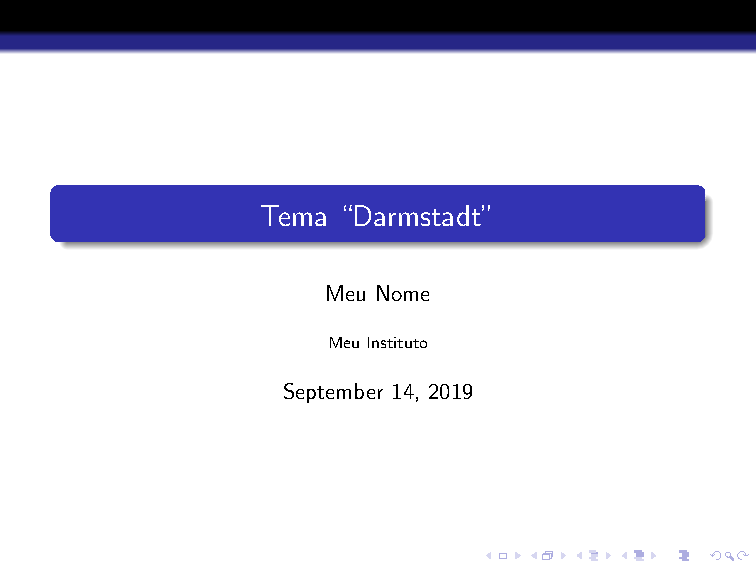
\includegraphics[scale=0.28,page=1]{./figs/beamer.pdf}
\tcbitem[squeezed title={Dresden}]    \centering \includegraphics[scale=0.28,page=2]{./figs/beamer.pdf}
\tcbitem[squeezed title={Frankfurt}]  \centering \includegraphics[scale=0.28,page=3]{./figs/beamer.pdf}
\tcbitem[squeezed title={Goettingen}] \centering \includegraphics[scale=0.28,page=4]{./figs/beamer.pdf}
\tcbitem[squeezed title={Hannover}]   \centering \includegraphics[scale=0.28,page=5]{./figs/beamer.pdf}
\tcbitem[squeezed title={Ilmenau}]    \centering \includegraphics[scale=0.28,page=6]{./figs/beamer.pdf}
\tcbitem[squeezed title={JuanLesPins}]\centering \includegraphics[scale=0.28,page=7]{./figs/beamer.pdf}
\tcbitem[squeezed title={Luebeck}]    \centering \includegraphics[scale=0.28,page=8]{./figs/beamer.pdf}
\tcbitem[squeezed title={Madrid}]     \centering \includegraphics[scale=0.28,page=9]{./figs/beamer.pdf}
\tcbitem[squeezed title={Malmoe}]     \centering \includegraphics[scale=0.28,page=10]{./figs/beamer.pdf}
\tcbitem[squeezed title={AnnArbor}]   \centering \includegraphics[scale=0.28,page=11]{./figs/beamer.pdf}
\tcbitem[squeezed title={Marburg}]    \centering \includegraphics[scale=0.28,page=12]{./figs/beamer.pdf}
\tcbitem[squeezed title={Montpellier}]\centering \includegraphics[scale=0.28,page=13]{./figs/beamer.pdf}
\tcbitem[squeezed title={PaloAlto}]   \centering \includegraphics[scale=0.28,page=14]{./figs/beamer.pdf}
\tcbitem[squeezed title={Pittsburg}]  \centering \includegraphics[scale=0.28,page=15]{./figs/beamer.pdf}
\tcbitem[squeezed title={Rochester}]  \centering \includegraphics[scale=0.28,page=16]{./figs/beamer.pdf}
\tcbitem[squeezed title={Singapore}]  \centering \includegraphics[scale=0.28,page=17]{./figs/beamer.pdf}
\tcbitem[squeezed title={Szeged}]     \centering \includegraphics[scale=0.28,page=18]{./figs/beamer.pdf}
\tcbitem[squeezed title={Warsaw}]     \centering \includegraphics[scale=0.28,page=19]{./figs/beamer.pdf}
\tcbitem[squeezed title={Antibes}]    \centering \includegraphics[scale=0.28,page=20]{./figs/beamer.pdf}
\tcbitem[squeezed title={Bergen}]     \centering \includegraphics[scale=0.28,page=21]{./figs/beamer.pdf}
\tcbitem[squeezed title={Berkeley}]   \centering \includegraphics[scale=0.28,page=22]{./figs/beamer.pdf}
\tcbitem[squeezed title={Berlin}]     \centering \includegraphics[scale=0.28,page=23]{./figs/beamer.pdf}
\tcbitem[squeezed title={Boadilla}]   \centering \includegraphics[scale=0.28,page=24]{./figs/beamer.pdf}
\tcbitem[squeezed title={CambridgeUS}]\centering \includegraphics[scale=0.28,page=25]{./figs/beamer.pdf}
\tcbitem[squeezed title={Copenhagen}] \centering \includegraphics[scale=0.28,page=26]{./figs/beamer.pdf}

\end{tcbitemize}

\end{texexptitled}

%\end{landscape}

\begin{marker}
Veja mais opções de temas, estilos e combinações do \textit{Beamer} em \url{https://hartwork.org/beamer-theme-matrix/}.
\end{marker}

\subsection{Ambientes especiais}
\label{sec:estrut_slide}

Em um \textit{frame} do \textit{Beamer}, podem ser inseridas listas, tabelas, imagens, equações e outros ambientes que já foram mostrados no Capítulo \ref{cap:parteII}. Além destes ambientes, o \textit{Beamer} suporta ambientes especiais que podem ser utilizados para destacar as informações inseridas. Um destes ambientes especiais, é o ambiente \mintinline{latex}{block}. Veja no Exemplo \ref{exe:beamer_block} a seguir como inserí-lo em um \textit{frame} do \textit{Beamer}:

\begin{texexptitled}[breakable,center lower,enhanced jigsaw,middle=2mm,listing side comment,righthand width=5.5cm,compilable listing,run latex,run dvips,run ps2pdf,pdf comment,comment style={raster columns=1},freeze pdf]{Ambiente {\tt block} em um \textit{frame} do \textit{Beamer}}{exe:beamer_block}
\documentclass{beamer}
\usepackage[utf8]{inputenc}

\usetheme{Warsaw}
	
\title{Título}
\author{Nome}
\date{September 2019}
	
\begin{document}
		
\maketitle
		
\section{Minha Seção}
		
\subsection{Minha Subseção}
		
\begin{frame}{Meu Frame}

    \begin{block}{Meu block}
        À noite, vovô Kowalsky vê o ímã cair no pé do pinguim queixoso e vovó põe açúcar no chá de tâmaras do jabuti feliz. 
    \end{block}

\end{frame}
	
\end{document}
\end{texexptitled}

\subsection{Transições e Animações}
\label{sec:trans_anima}

Efeitos de transição e animações também podem ser utilizadas em um documento \textit{Beamer}. Entretanto, observe que, diferentemente do \textit{Microsoft PowerPoint}, estes efeitos e animações são como as animações feitas em \textit{flipboards}, i.e., animações quadro-a-quadro. Isso significa que vários \textit{frames} (ou \textit{slides}) são produzidos até que a animação ou o efeito final seja alcançado. Veja no Exemplo \ref{exe:beamer3} como os itens de uma lista são apresentados de forma que apenas o item atual esteja realçado. Este efeito é muito comum e recebe o nome de pausa e ele é obtido a partir do comando \mintinline{latex}{\pause}.

% Ref. dos exemplos: http://web.mit.edu/rsi/www/pdfs/beamer-tutorial.pdf

\begin{texexptitled}[breakable,center lower,enhanced jigsaw,middle=2mm,listing side comment,righthand width=5.5cm,compilable listing,run latex,run dvips,run ps2pdf,pdf comment,comment style={raster columns=1},freeze pdf]{Adicionando pausas no \textit{Beamer} com o comando {\tt pause}}{exe:beamer3}
\documentclass{beamer}
\usepackage[utf8]{inputenc}

\usetheme{AnnArbor}

\title{Título}
\author{Nome}
\date{September 2019}

\begin{document}

\maketitle

\section{Minha Seção}

\subsection{Minha Subseção}

\begin{frame}{Meu Frame}
Minha Lista:
\begin{itemize}
    \pause
    \item Item 1
    \pause
    \item Item 2
    \pause
    \item Item 3
\end{itemize}
\end{frame}

\end{document}
\end{texexptitled}

Observe no Exemplo \ref{exe:beamer3} que os itens da lista são adicionados um após o outro de forma sequencial. Este comportamento pode ser alterado de forma que a ordem em que os itens aparecem possa ser controlada. Compare o Exemplo \ref{exe:beamer3} com o Exemplo \ref{exe:beamer4} a seguir:

\begin{texexptitled}[breakable,center lower,enhanced jigsaw,middle=2mm,listing side comment,righthand width=5.5cm,compilable listing,run latex,run dvips,run ps2pdf,pdf comment,comment style={raster columns=1},freeze pdf]{Controlando itens em uma lista no \textit{Beamer}}{exe:beamer4}
\documentclass{beamer}
\usepackage[utf8]{inputenc}

\usetheme{CambridgeUS}

\title{Título}
\author{Nome}
\date{September 2019}

\begin{document}

\maketitle

\section{Minha Seção}

\subsection{Minha Subseção}

\begin{frame}{Meu Frame}
Minha Lista:
\pause
\begin{itemize}
    \item<2-> Item 1
    \item<3-> Item 2
    \item<4-> Item 3
\end{itemize}
\end{frame}

\end{document}
\end{texexptitled}

No Exemplo \ref{exe:beamer4}, não foi utilizando o comando \mintinline{latex}{\pause} e, ao invés dele, foram adicionados parâmetros ao comando \mintinline{latex}{\item} de forma que fosse especificado em qual \textit{slide} aquela informação da lista deve aparecer. Dessa forma, o comando \mintinline{latex}{\item<2-> Item 1} deve aparecer apenas no \textit{slide} número 2, o item descrito pelo comando \mintinline{latex}{\item<3-> Item 2} deve aparecer apenas no slide número 3 e assim por diante. Além disso, observe que há um sinal de {\tt -} (menos) após o número do \textit{slide}, indicando que aquele item irá aparecer a partir do número do \textit{slide} indicado (e em diante). Na Tabela \ref{tab:beamer1} estão listados alguns dos comandos de controle dos elementos de um \textit{slide} do \textit{Beamer}.

\begin{table}[H]
\centering
\caption{Alguns comandos de controle dos elementos de um \textit{slide} do \textit{Beamer}.}
\label{tab:beamer1}
    \begin{tabular}{p{3cm}p{8cm}}
    \toprule
    \textbf{Comando} & \textbf{Descrição} \\
    \midrule
    \mintinline{latex}{\textbf<>{}} & Controla quando um texto deverá ocorrer em negrito \\
    \mintinline{latex}{\textit<>{}} & Controle quando um texto deverá ocorrer em itálico \\
    \mintinline{latex}{\color<>{}} & Controla quando um texto deverá ocorrer em uma cor diferente \\
    \mintinline{latex}{\alert<>{}} & Controla quando um texto deverá ocorrer destacadamente \\
    \bottomrule
    \end{tabular}
\FONTE{Produção do autor.}
\end{table}

% Acho que esta seção deve vir antes 
%\subsection{Elementos dos Slides}
%\label{sec:elem_slides}

%ambiente block

%\section{Pacote TColorBox}
%\label{sec:tcolorbox}

%Se você chegou até esta seção lendo todo o documento, deve ter percebido que todos os exemplos, dicas e exercícios foram colocados dentro de caixas coloridas para destacá-los. Estas caixas são fornecidas pelo pacote {\tt tcolorbox}. O pacote {\tt tcolorbox} é um pacote muito interessante de ser utilizado. Com ele é possível também produzir pôsteres em qualquer formato.% Os elementos do texto que contém dicas, comandos, exemplos e exercícios que se encontram neste documento, foram todos produzidos utilizando este pacote. Com ele é possível também produzir pôsteres em qualquer formato.

%As informações e instruções apresentadas nesta seção, não buscam esgotar a utilização do pacote {\tt tcolorbox}, mas apresenta, de forma sucinta, um meio objetivo de utilizá-lo para a produção de pôsteres, objetivo que também pode ser cumprido com o pacote {\tt beamer}.

%\section{Confecção de Pôsteres e Apresentações}
%\subsection{Estilos, equações, gráficos e tabelas}

%\section{Apresentações}
%\subsection{Construção de figuras e diagramas, pequenas animações e configurações especiais}

%\section{Pôsteres}
%\subsection{Definindo estilos}

%\begin{dica}{Dica \#n}
%É possível também utilizar o pacote \mintinline{latex}{tcolorbox} para fazer pôsteres também!
%\end{dica}
%\begin{marker}
%É possível também utilizar o pacote %\mintinline{latex}{tcolorbox} para fazer pôsteres também!
%\end{marker}

% https://tex.stackexchange.com/questions/486009/tcolorboxes-side-by-side

%\subsection{Outros pacotes para apresentações e pôsteres}
%\label{sec:outrospacs}

\begin{marker}
No \LaTeX{} há outros pacotes que podem ser utilizados para a confecção de apresentações e pôsteres no estilo do \textit{Microsoft PowerPoint}. Entre eles, destacam-se a classe {\tt powerdot} que fornece estilos muito semelhantes àqueles que podem ser encontrados no \textit{Microsoft PowerPoint} e o pacote {\tt tcolorbox}.
\end{marker}